\chapter{Monte Carlo Simulations}
\label{cha:MonteCarlo}
%
$\phi_h$ distributions at CLAS are highly dependent on acceptance.
Here, acceptance refers to both geometrical acceptance (the location of active detector elements) and the efficiency in the active regions.
The $cos\phi_h$ and $cos2\phi_h$ moments, therefore, cannot be extracted without acceptance corrections.
This is done using Monte Carlo simulations.
An event generator is used to create a realistic large set of events (several iterations may be required before the set is ``realistic'') which are passed through a GEANT based simulation of the CLAS detector.
For a given kinematic space, the acceptance is equal to the number of reconstructed events divided by the number of generated events.
The number of events in the E1-f data is then divided by the acceptance to get a corrected value for the number of events.
%
\section{Simulation}
\label{sec:Simulation}
%
Below is a general outline for how the simulations are performed.
The details for each step will be discussed in the subsequent subsections.
\begin{itemize}
\item clasDIS is a program that generates electron-proton scattering events.
\item GSim is a program that attempts recreate how CLAS would reconstruct the generated events.
\item GPP (GSim Post Processing) is a program that smears and introduces additional inefficiencies to the GSim results to make the resolutions and acceptance more realistic.
\item the RECSIS software cooks and formats the raw data using the same procedure as in the E1-f cooking and formatting.
\item the same particle ID and fiducial cuts used in the E1-f data are used on the simulation.
\end{itemize}
%
\subsection{Event Generation}
\label{subsec:EventGeneration}
%
The first step in doing Monte Carlo simulations is event generation.
The distribution of events created by the generator should resemble nature as closely as possible.
Since the $cos\phi_h$ and $cos2\phi_h$ moments are not known a priori, this is accomplished in an iterative way, starting with a flat $\phi_h$ distribution (i.e. $A^{cos\phi_h}_{UU} = A^{cos2\phi_h}_{UU} = 0$).
The program used to do this is clasDIS, which is based on the PYTHIA generator and has been modified to be compatible with the kinematics at CLAS.
The control options used with clasDIS for this analysis are summarized in table~\ref{tab:clasDIScontrolOpts}.
Approximately one billion events were generated in order to minimize the statistical error of the acceptance calculations.
%
\begin{table}[htp]
\centering
\begin{tabular}{ p{4cm} p{10cm} }
\hline
\textbf{Option} & \textbf{Description} \\ \hline
--trig N & Tells the generator to process N events. \\
--datf & Tells the generator to output a data file. \\
--outform 2 & Tells the generator to format the output for GSim. \\
--beam 5498 & Sets the beam energy to 5.498 GeV. \\
--zpos -250 & Sets the z-position at -250 mm. \\
--zwidth 25 & Sets the target half-width to 25 mm. \\
--t 5 60 & Sets the range of acceptable $\theta$ in degrees. \\
--parl3 0.7 & Sets the mean of the $k_T$ distribution, which is tuned such that the output $P_{h\perp}$ matches E1-f. \\
--lst15 145 & Defines the set of parton distribution functions used in the simulation. \\
--parj33 0.3 & Defines the remaining energy below which the fragmentation of a parton system is stopped and two hadrons are formed. \\
\hline
\end{tabular}
\caption{Control options for the clasDIS event generator.}
\label{tab:clasDIScontrolOpts}
\end{table}
%
\subsection{Detector Simulation}
\label{subsec:DetectorSimulation}
%
The software package used to simulate the CLAS detector is GSim.
GSim is a GEANT based Monte Carlo simulation that simulates the passage of particles through matter.
The functionality includes detector geometry, physics models, and particle tracking and hits.
Each event generated with clasDIS is passed to GSim; GSim then produces a realistic reconstruction of how the CLAS detector would reconstruct those events.
Figure~\ref{fig:gsim_int_5events} shows an example of this.
Both the generated information and the reconstructed information of the event are saved in the GSim output data file, the reconstructed portion being identical in format to the E1-f raw data files.

Each experimental run at Jefferson Lab uses slightly different conditions (magnetic field strength, target type/polarization, etc.).
To customize GSim to be compatible with a particular run, a file called ffread.in must included in the GSim options.
The ffread.in file for the E1-f run is summarized in table~\ref{tab:ffread_table}
%
\begin{figure}[htp]
\centering
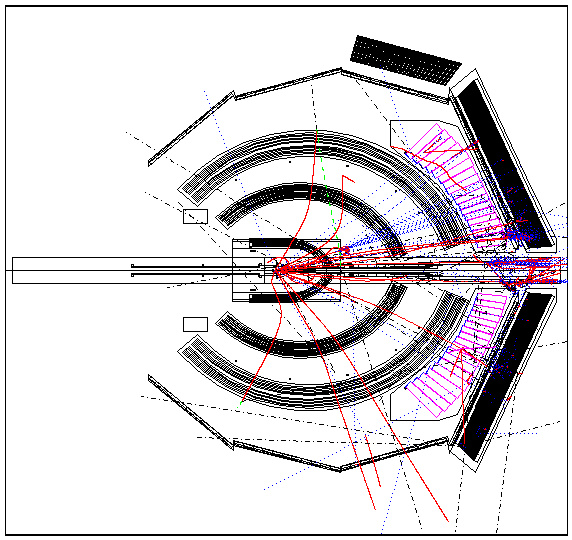
\includegraphics[width=4in]{figures/gsim_int_5events.png}
\caption{A GSim reconstruction of five simulated events. The red tracks represent charged particles while gray tracks represent neutral particles.}
\label{fig:gsim_int_5events}
\end{figure}

\begin{center}
\begin{longtable}{l l}
\caption{The information contained in the ffread.in file, customized for the E1-f run.}\\
\hline
\textbf{Input} & \textbf{Description} \\
\hline
\endfirsthead
\multicolumn{2}{c}%
{\tablename\ \thetable\ -- \textit{Continued from previous page}} \\
\hline
\textbf{Input} & \textbf{Description} \\
\hline
\endhead
\hline \multicolumn{2}{r}{\textit{Continued on next page}} \\
\endfoot
\hline
\endlastfoot
GEOM \lq ALL\rq & Includes all CLAS geometry. \\
NOGEOM \lq PTG\rq \lq ST\rq \lq IC\rq & Excludes geometry not present in E1-f. \\
MAGTYPE 3 & \parbox[t]{7cm}{Sets magnetic field type to ``torus + mini from lookup table.''} \\ %parbox prevents the long sentence from running off the edge of the page
CUTS 5.e-3 5.e-3 5.e-3 5.e-3 & Kinetic energy cuts in GeV. \\
CCCUTS 1.e-3 1.e-3 1.e-3 1.e-3 & Cuts for the \v{C}erenkov counter. \\
DCCUTS 1.e-4 1.e-4 1.e-4 1.e-4 & Cuts for the drift chamber. \\
ECCUTS 1.e-4 1.e-4 1.e-4 1.e-4 & Cuts for the electromagnetic calorimeter. \\
SCCUTS 1.e-4 1.e-4 1.e-4 1.e-4 & Cuts for the time-of-flight detector. \\
NTARGET 2 & Sets the target type to liquid hydrogen. \\
MAGSCALE 0.5829 0.7495 & Sets the scale of the magnetic fields. \\
RUNG 10 & Default setting. \\
TARGET \lq e1e\rq & \parbox[t]{7cm}{Defines the target geometry (e1e is compatible with e1f).} \\
TGMATE \lq PROT\rq \lq ALU\rq & Sets the target and target cell materials. \\
TGPOS 0.00 0.00 -25.0 & Defines the target position. \\
NOMCDATA \lq ALL\rq & \parbox[t]{7cm}{Default setting to turn off additional GEANT hit information.} \\
SAVE \lq ALL\rq \lq LEVL\rq 10 & Save all secondaries up to cascade level 10. \\
KINE 5 & Setting for LUND event generator. \\
AUTO 1 & \parbox[t]{7cm}{Automatic computation of the tracking medium parameters.} \\
STOP & GEANT command to end the ffread file.
\label{tab:ffread_table}
\end{longtable}
\end{center}
%
\subsection{Resolution Matching}
\label{subsec:ResolutionMatching}
%
Since GSim significantly over estimates the detector resolution, the GPP program is used to smear the DC and TOF values.
To determine the amount of DC smearing necessary, studies were done using the reaction $ep \rightarrow e\pi^+ \pi^- p$ in the experimental data and in the Monte Carlo.
After selecting these events, the following resolutions are defined
%
\begin{equation}
\label{eq:resolutionDefinitions}
\begin{split}
\Delta p_{\pi^+} &= p_{\pi^+, calc} - p_{\pi^+, rec} \\
\Delta \theta_{\pi^+} &= \theta_{\pi^+, calc} - \theta_{\pi^+, rec} \\
\Delta \phi_{\pi^+} &= \phi_{\pi^+, calc} - \phi_{\pi^+, rec} \\
\end{split}
\end{equation}
%
where $p$, $\theta$, and $\phi$ are the momentum, $\theta$, and $\phi$ in the lab frame and the $\pi^+, rec$ subscript refers to the actual reconstructed value of the $\pi^+$ while $\pi^+, calc$ is the value calculated based on the momenta of the other three particle and momentum conservation.
These resolutions can be compared for data and simulation and the simulation can be tuned with GPP until the resolutions match.
This tuning is done with three parameters called ``a'', ``b'', and ``c.''
The optimum values for this analysis were found to be $a = b = c = 2.5$.
Comparison between the data and the Monte Carlo with these parameters can be seen in figures~\ref{fig:DeltapRes_dataAndMC}, \ref{fig:DeltaThetaRes_dataAndMC}, and~\ref{fig:DeltaPhiRes_dataAndMC}.
%
\begin{sidewaysfigure}[htp]
\centering
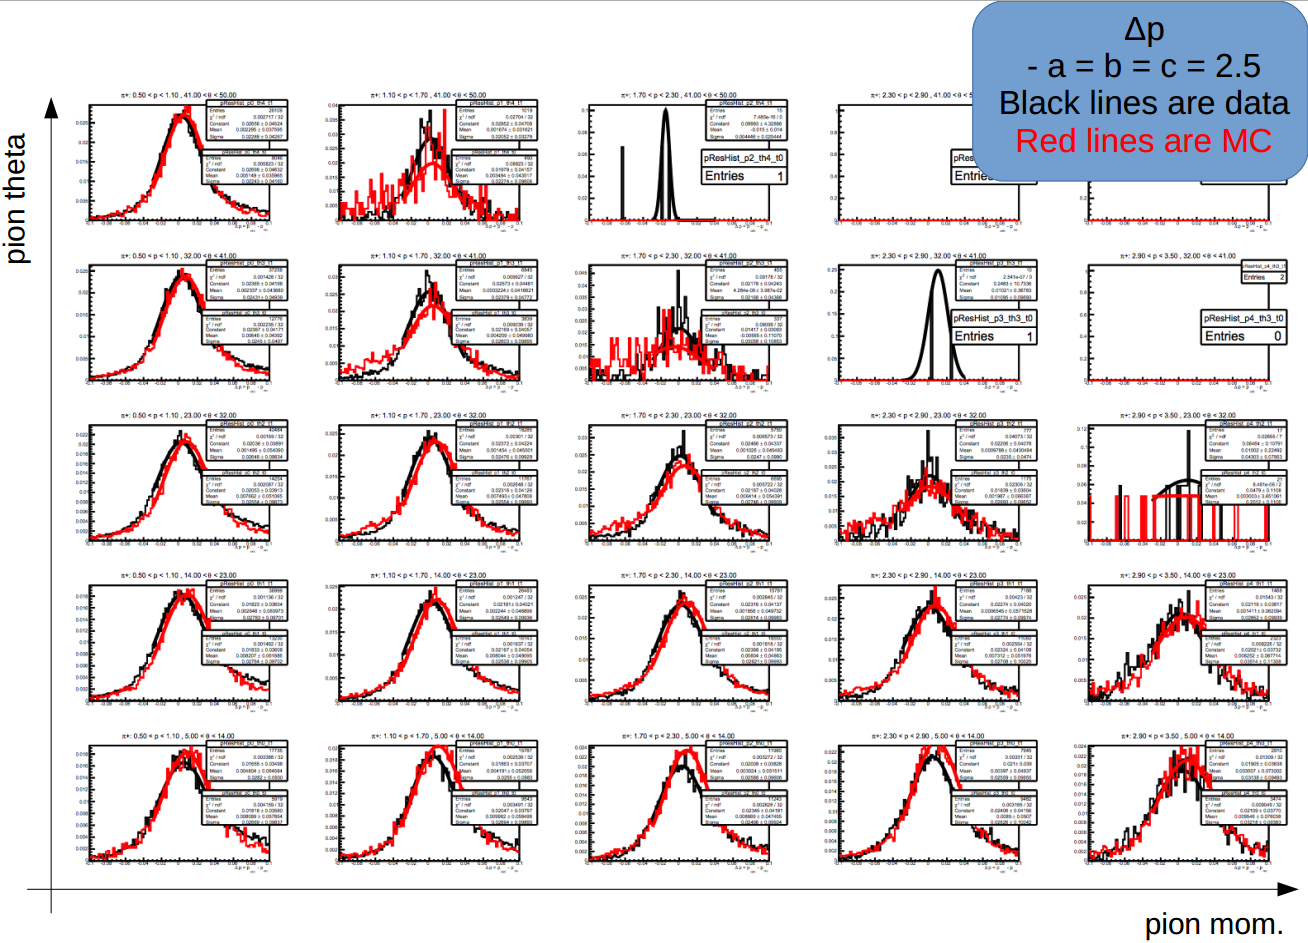
\includegraphics[width=8.5in]{figures/DeltapRes_dataAndMC.png}
\caption{$\Delta p_{\pi^+}$ in bins of $\pi^+$ $\theta$ and $\phi$ for data (black) and Monte Carlo with GPP parameters $a = b = c = 2.5$ (red). It is clear that the agreement in resolution is good between the data and Monte Carlo.}
\label{fig:DeltapRes_dataAndMC}
\end{sidewaysfigure}
%
\begin{sidewaysfigure}[htp]
\centering
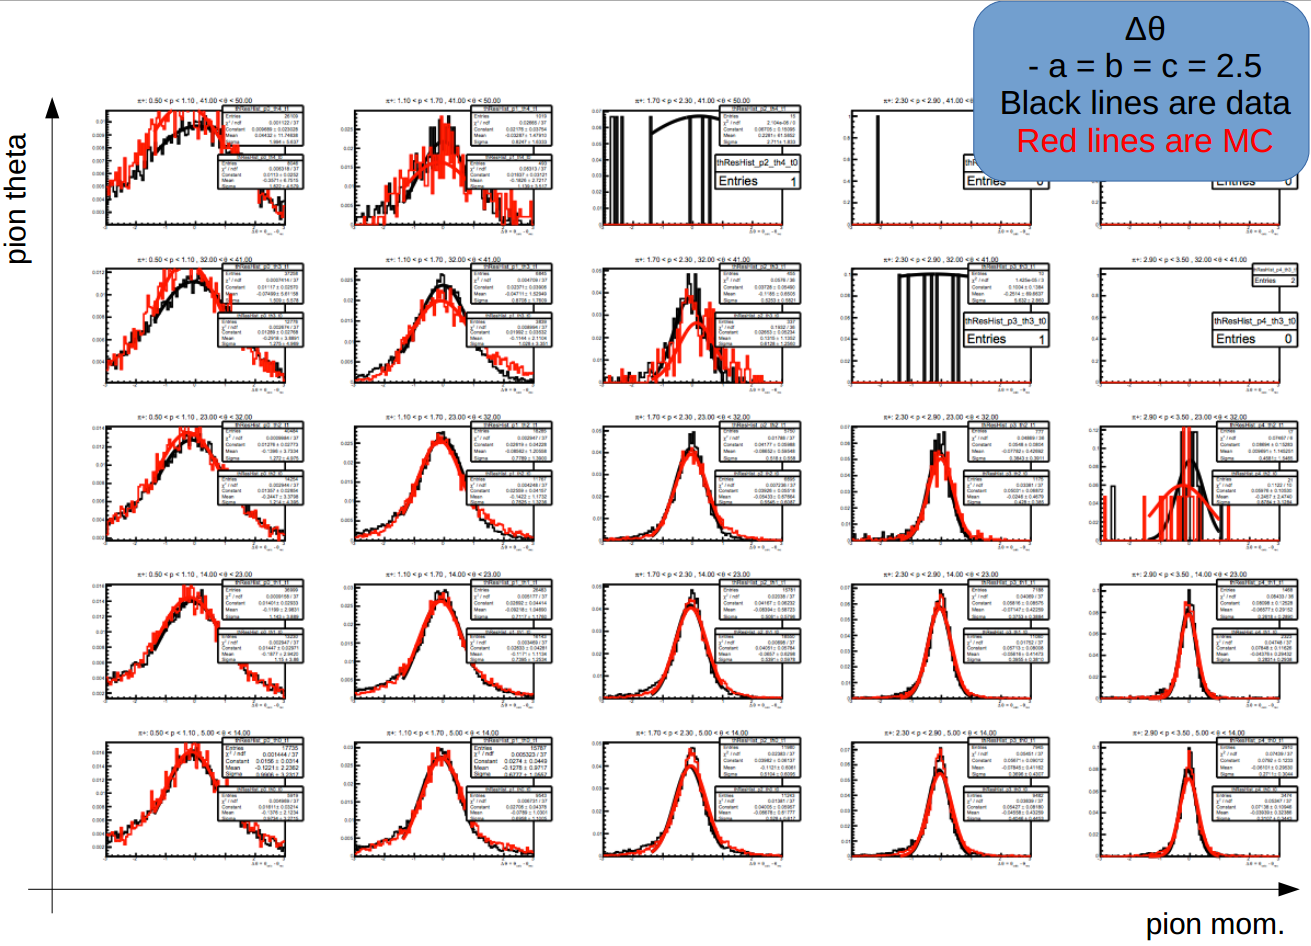
\includegraphics[width=8.5in]{figures/DeltaThetaRes_dataAndMC.png}
\caption{$\Delta \theta_{\pi^+}$ in bins of $\pi^+$ $\theta$ and $\phi$ for data (black) and Monte Carlo with GPP parameters $a = b = c = 2.5$ (red). It is clear that the agreement in resolution is good between the data and Monte Carlo.}
\label{fig:DeltaThetaRes_dataAndMC}
\end{sidewaysfigure}
%
\begin{sidewaysfigure}[htp]
\centering
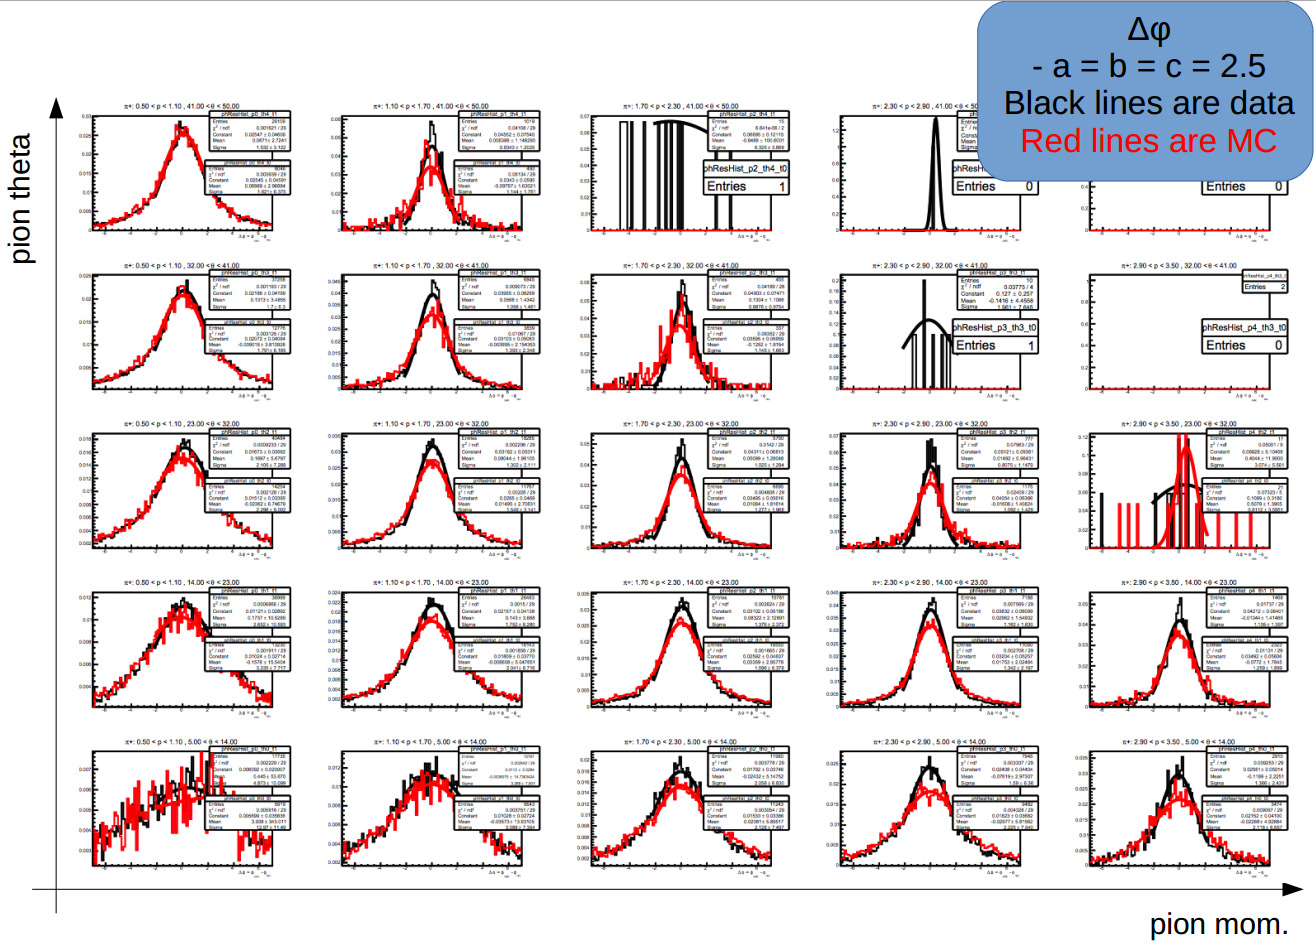
\includegraphics[width=8.5in]{figures/DeltaPhiRes_dataAndMC.png}
\caption{$\Delta \phi_{\pi^+}$ in bins of $\pi^+$ $\theta$ and $\phi$ for data (black) and Monte Carlo with GPP parameters $a = b = c = 2.5$ (red). It is clear that the agreement in resolution is good between the data and Monte Carlo.}
\label{fig:DeltaPhiRes_dataAndMC}
\end{sidewaysfigure}
%

GPP also smears the TOF values via a parameter ``f.''
The f parameter can be tuned by comparing the widths of the $\beta$ distributions (in bins of momentum) for data and Monte Carlo.
It was found that $f = 0.85$ is the best value for this analysis.
Figure~\ref{fig:TOFres_dataAndMC} compares $\pi^+$ $\beta$ for data and Monte Carlo with $f = 0.85$.
%
\begin{sidewaysfigure}[htp]
\centering
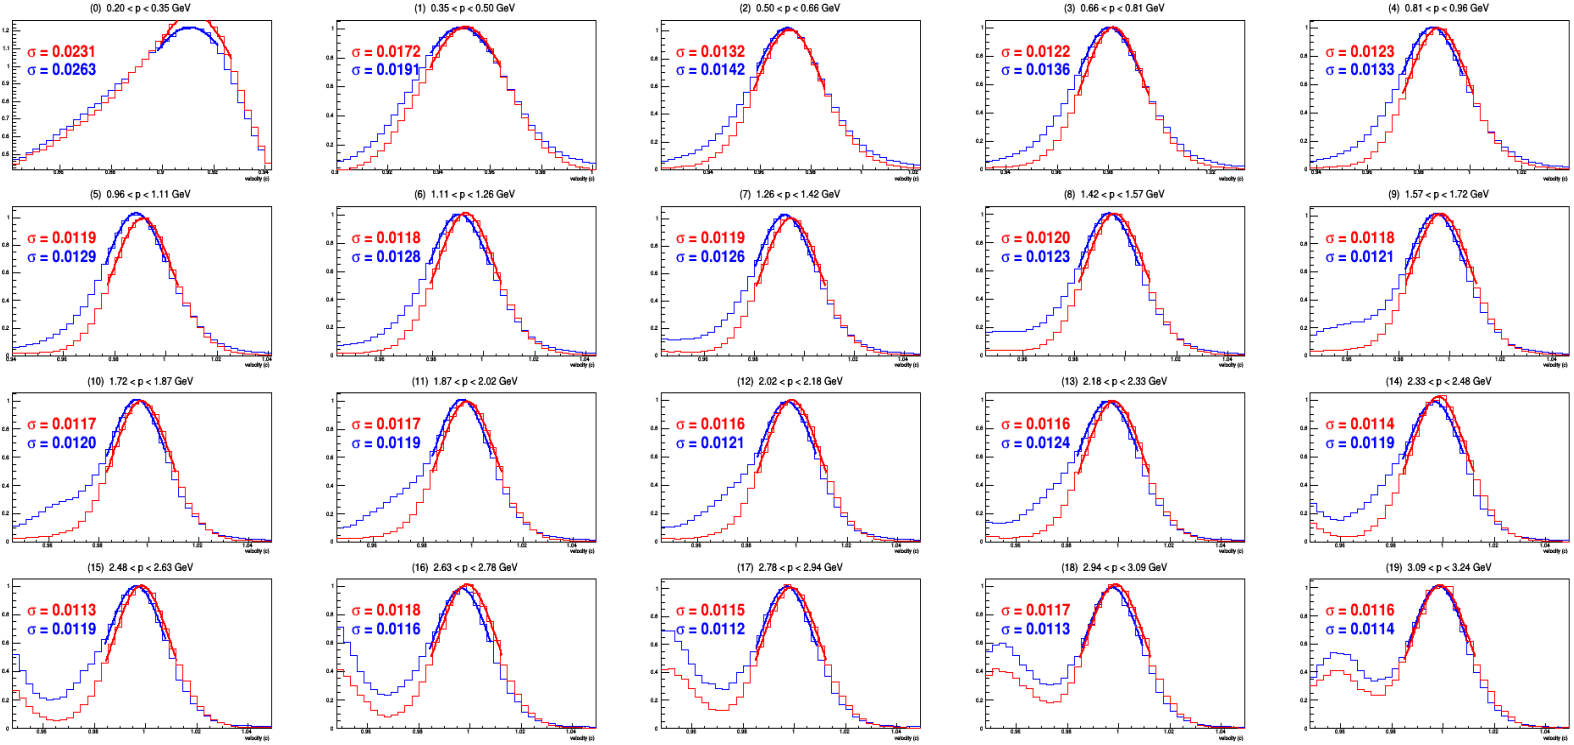
\includegraphics[width=8.5in]{figures/TOFres_dataAndMC.png}
\caption{$\pi^+$ $\beta$ distributions in bins of momentum for data (blue) and Monte Carlo with $f = 0.85$ (red). The top left plot is the lowest momentum bin and the bottom right plot is the highest momentum bin. Each peak is fit with a gaussian and $\sigma$ is printed on the plot (MC on top, data on bottom). This shows the good agreement in TOF resolution between the data and Monte Carlo.}
\label{fig:TOFres_dataAndMC}
\end{sidewaysfigure}
%

The second purpose of GPP is to cut or introduce inefficiencies to certain DC wires in the simulation so that it matches the data.
To check that this worked properly a wire map of the DC occupancy is made for the data and simulation (after using GPP).
This is shown in figure~\ref{fig:DCoccupancy} which confirms the efficacy of this feature of GPP.
%
\begin{sidewaysfigure}[htp]
\centering
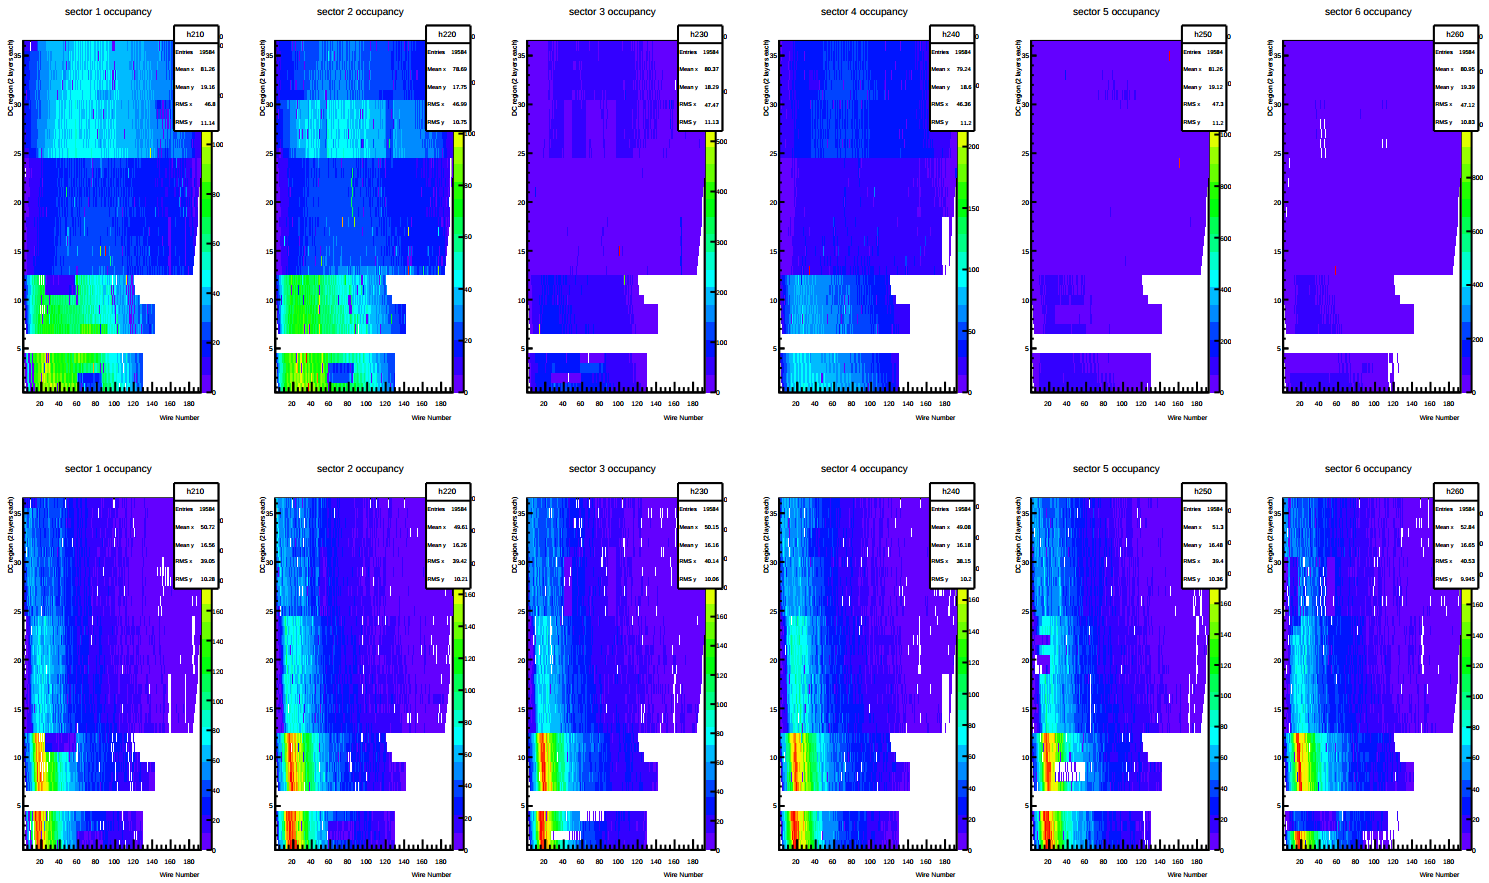
\includegraphics[width=8.5in]{figures/DCoccupancy.png}
\caption{A wire map of the DC occupancy for data (top row) and Monte Carlo (bottom row) for each sector (column 1 is sector 1, column 2 is sector 2, etc.). The holes are consistent between data and Monte Carlo confirming the efficacy of GPP.}
\label{fig:DCoccupancy}
\end{sidewaysfigure}
%

\subsection{Monte Carlo Reconstruction and Event Selection}
\label{subsec:ReconstructionAndEventSelection}
%
After the generated data has been passed through GSim and after the GSim output has been modified by GPP, this data is then cooked with RECSIS in the same was as the experimental data.
This produces an ntuple file where each event has a generated part and (possibly) a reconstructed part, the reconstructed part being identical in format to the cooked E1-F data files.
The reconstructed part is put through the same set of particle ID and fiducial cuts as the experimental data.
The cuts used here are not necessarily exactly identical to the experimental cuts, but they are the same kind of cuts; for example a $\mu \pm 3\sigma$ cut could produce slightly different cut values if $\mu$ and $\sigma$ are slightly different in the data and simulation.
Figure~\ref{fig:MC_pip_vvpCut} shows, as an example, the momentum dependent $\beta$ cut for $\pi^+$ ID for the reconstructed Monte Carlo; this should be compared to the experimental data version in figure~\ref{fig:pip_vvpCut}.
Finally, both the generated and reconstructed Monte Carlo data is orgainzed into bins of $x$, $Q^2$, $z$, $P_{h\perp}^2$, and $\phi_h$ in the same way the data is.
%
\begin{figure}[htp]
\centering
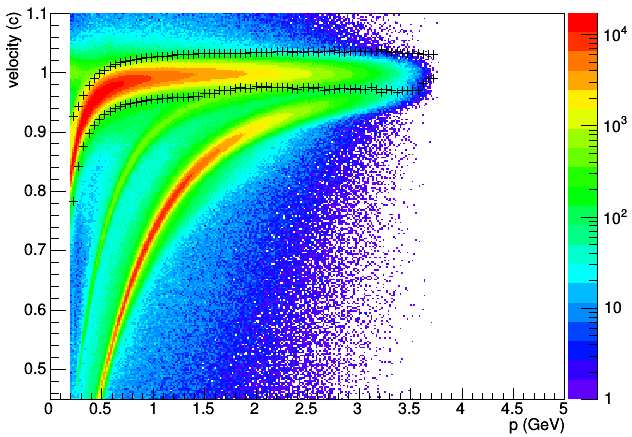
\includegraphics[width=4in]{figures/MC_pip_vvpCut.png}
\caption{The two dimensional view of the momentum dependent $\pi^+$ $\beta$ cut for the reconstructed Monte Carlo. This should be compared to the experimental data version in figure~\ref{fig:pip_vvpCut}.}
\label{fig:MC_pip_vvpCut}
\end{figure}
%
%
%%%%%%%%%%%%%%%%%%%%%%%%%%%%%%%%%%%%%%%%%%%%%%%%
%%%%%%%%%%%%%%%%%%%%%%%%%%%%%%%%%%%%%%%%%%%%%%%%

\clearpage % should prevent a backlog of figures from piling up

\section{Minimum $\phi_h$ Coverage for Reliable Fitting}
\label{sec:minPhihCoverage}
There are certain regions of phase space where the CLAS acceptance is zero.
These regions commonly occur around $\phi_h = 0$, potentially creating an occasion for unreliable results when fitting a particular $\phi_h$ distribution.
A study is therefore needed to check what is the minimum allowable coverage in $\phi_h$ for which $A_0$, $A_{UU}^{\cos\phi_h}$, and $A_{UU}^{\cos 2\phi_h}$ can be reliably extracted.
The criteria for $A_0$ will be different than the criteria for $A_{UU}^{\cos\phi_h}$ and $A_{UU}^{\cos 2\phi_h}$ since $A_0$ is a much more stable quantity.

This study consisted of generating $\phi_h$ distributions with three options: the number of events to generate, the value of the $\cos\phi_h$ moment, and the value of the $\cos 2\phi_h$ moment.
The generated values of $A_{UU}^{\cos\phi_h}$ were -0.3, -0.2, -0.1, 0.0, 0.1, 0.2, and 0.3 (7 values).
Similarly, the generated values of $A_{UU}^{\cos 2\phi_h}$ were -0.3, -0.2, -0.1, 0.0, 0.1, 0.2, and 0.3 (7 values).
Finally, the number of generated events were 500, 1000, 2000, 5000, 10000, 20000, 50000, 100000, and 1000000 (9 values).
All $7 \times 7 \times 9 = 441$ combinations were produced.
Each distribution is then fit several times; each time a different range of $\phi_h$ around $0$ was first cut out.
An example of this can be seen in figure~\ref{fig:holeWidthStudyExample} which shows 5000 generated $\phi_h$ events with $A_{UU}^{\cos\phi_h} = -0.2$ and $A_{UU}^{\cos 2\phi_h} = 0.1$ and fit results; with each successive plot a larger range of $\phi_h$ around $0$ is cut out before fitting.
%
\begin{sidewaysfigure}[htp]
\centering
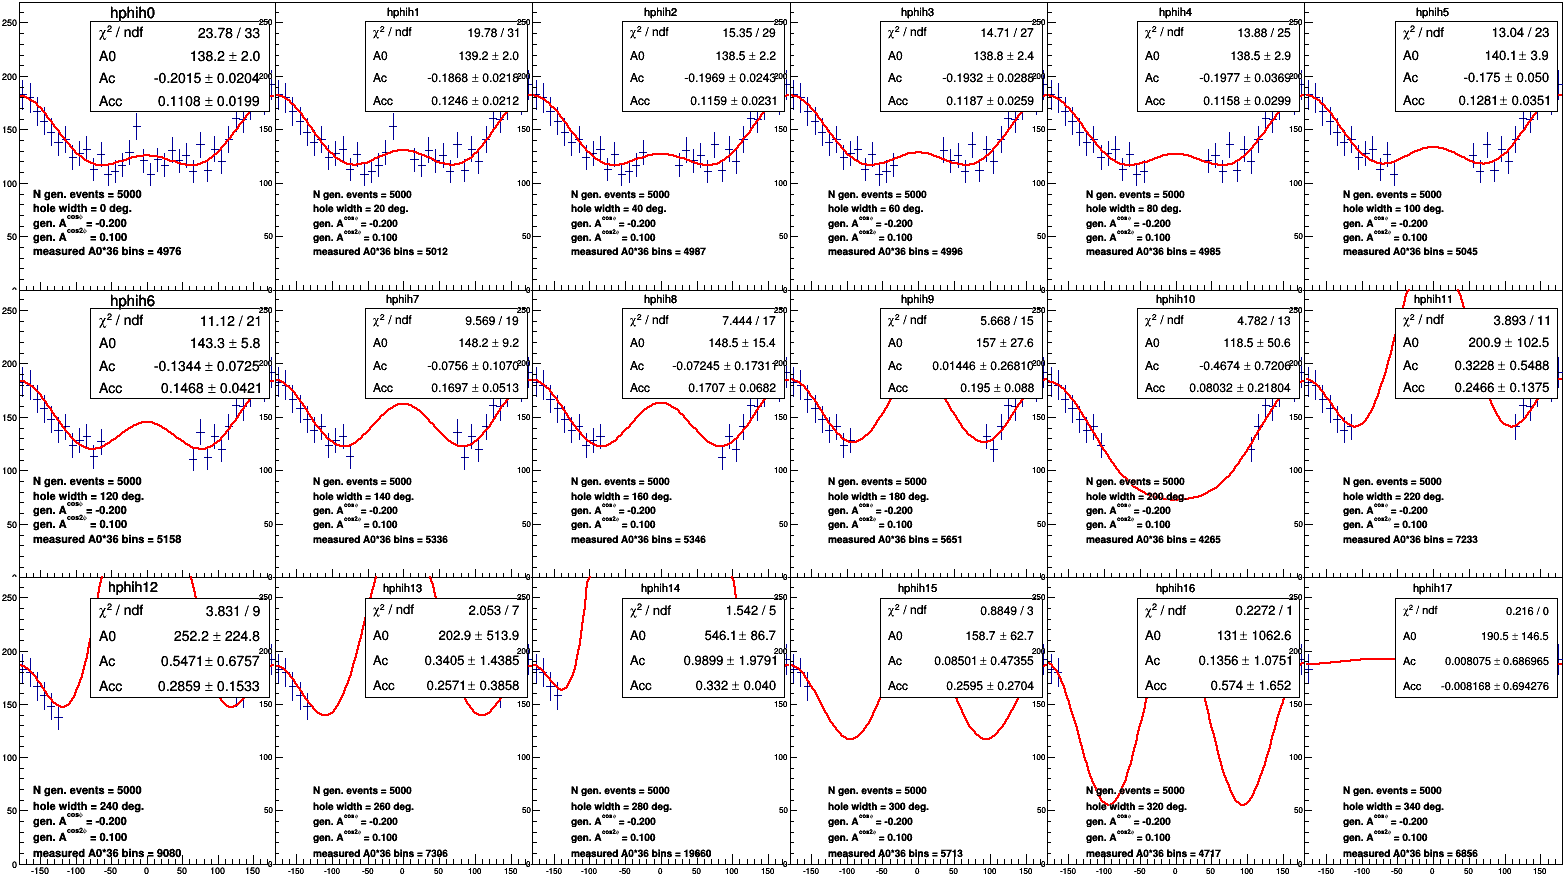
\includegraphics[width=8.5in]{figures/holeWidthStudyExample.png}
\caption{Generated $\phi_h$ distributions with fit results with different ranges of $\phi_h$ cut out around $0$. The top left plot has full $360^\circ$ coverage while the bottom right plot has only $10^\circ$ of coverage on each side. In this example 5000 events were generated with $A_{UU}^{\cos\phi_h} = -0.2$ and $A_{UU}^{\cos 2\phi_h} = 0.1$.}
\label{fig:holeWidthStudyExample}
\end{sidewaysfigure}

As expected, higher statistics distributions produce more stable fit results.
Within common sense limitations, a worst-case-scenario should be used as the criteria; anything less conservative could produce unreliable results.
Furthermore, generated distributions are always much more ideal than experimental results.
The case of 2000 generated events with $A_{UU}^{\cos\phi_h} = -0.2$ and $A_{UU}^{\cos 2\phi_h} = 0.0$ is used as a representative example.
The results for this case are summarized in figure~\ref{fig:holeWidthStudySummary}.
It is clear that the fit results become very volatile with a hole width greater than $60^\circ$ (i.e. events between $-30^\circ$ and $30^\circ$ are cut).
%
\begin{figure}[htp]
\centering
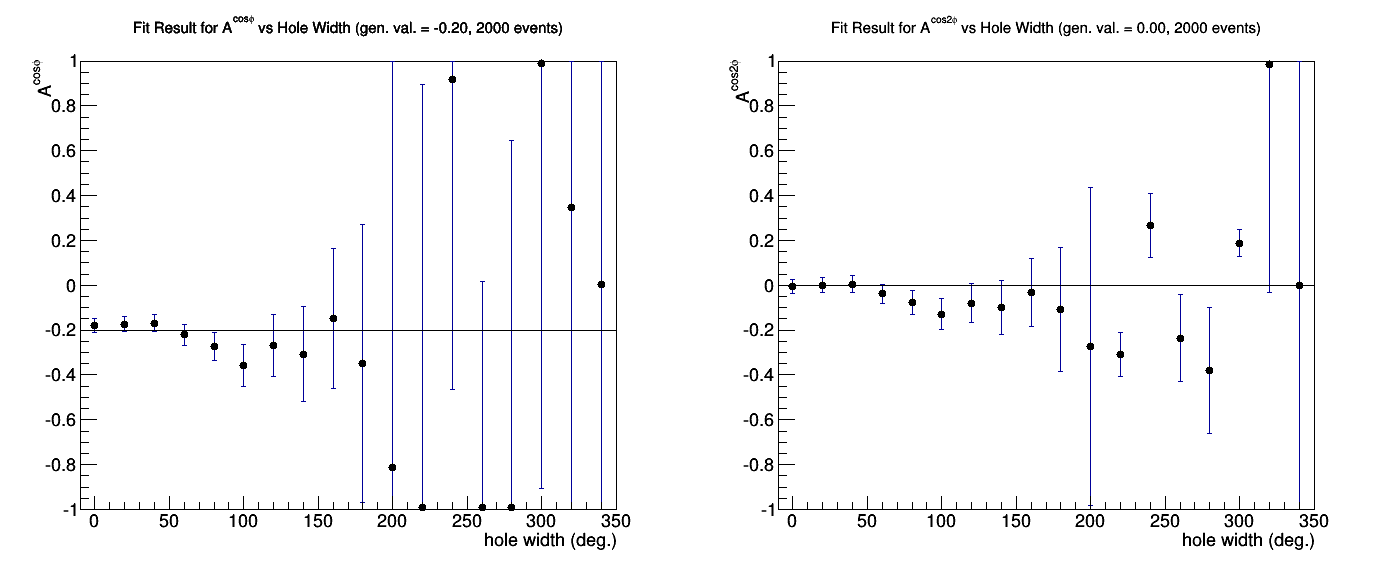
\includegraphics[width=6in]{figures/holeWidthStudySummary.png}
\caption{$A_{UU}^{\cos\phi_h}$ (left) and $A_{UU}^{\cos 2\phi_h}$ (right) extracted from the fit of the generated $\phi_h$ distribution as a function of the width of the zero acceptance hole. The black horizontal lines show the generated values.}
\label{fig:holeWidthStudySummary}
\end{figure}

As a result of this study, $A_{UU}^{\cos\phi_h}$ and $A_{UU}^{\cos 2\phi_h}$ are not measured in bins where there is an acceptance hole in $\phi_h$ greater than $60^\circ$ in width.
For measuring $A_0$, at least $100^\circ$ of coverage is required.

